\chapter{\textcolor{myred}{Simulaciones Computacionales}}

\section{\huge{Resolviendo las Geodésicas mediante Métodos Númericos}}

\textcolor{myred}{\hrule}
\begin{flushright}
\textit{What happens if a big asteroid hits Earth?\\Judging from realistic simulations involving a sledge hammer\\and a common laboratory frog, we can assume it will be pretty bad.\\\textbf{Dave Barry}}
\end{flushright}
 
\newthought{En los capítulos anteriores} vimos los conceptos, encontramos la métrica y derivamos las geodésicas. El trabajo está hecho, a partir de aquí solo jugaremos con las ideas que ya hablamos.



\newthought{El objetivo es simular la trayectoria} de objetos masivos con carga $q$, y de fotones, en los alrededores de un objeto esférico de masa $M$ y carga $Q$ utilizando el método de Runge-Kutta de 4to orden. Para eso recurrimos a las ecuaciones geodésicas (\ref{eqlightlike}), y (\ref{eqtimelikecargado}) y notamos dos inconvenientes:

\begin{itemize}
    \item Son ecuaciones diferenciales de primer orden, pero no son lineales.
    \item Nos hablan de $dr/d\phi$, lo cuál nos permitiría dibujar la órbita pero se pierde la noción de ''velocidad''\footnote{Para el caso de cuerpos con masa, nos referimos a las variaciones de las coordenadas, $t$, $r$ y $\phi$ respecto de el tiempo propio $\tau$. Para el caso de la luz, es más delicado porque sería importante definir una coordenada temporal específica.} del objeto.
\end{itemize}

Lo ideal sería contar con un conjunto de ecuaciones lineales de segundo orden de $r=r(\phi)$ para la órbita, y de las coordenadas $t=t(\tau)$, $r=r(\tau)$ y $\phi=\phi(\tau)$. Para estas últimas, podemos usar las Ecs. (\ref{eqt3.4}), (\ref{eqradial3.4}) y (\ref{eqazimutal3.4}) obtenidas del Lagrangiano de una partícula cargada en el espacio-tiempo de R-N. Idealmente, nuestra simulación nos permitiría animar la trayectoria de cuerpos con masa y carga, y dibujar la trayectoria cualquier cuerpo, incluso fotones. Animarla daría una noción de ''velocidad'', y dibujarla nos podría representar fenómenos físicos como la precesión de perihelios y afelios, las órbitas elípticas de planetas, como un agujero negro ''atrapa'' la luz, dilatación temporal en las cercanías de un campo gravitatorio intenso, etc.

\subsection*{\textbf{Ecuación general de la trayectoria de \textit{cosas} en la geometría R-N}}
Para obtener ecuaciones de segundo orden, hagamos lo más directo: derivemos las ecuaciones que tenemos. Empecemos con (\ref{eqtimelikecargado}):

\begin{equation}
\begin{split}
    \left( \frac{dr}{d\phi} \right)^2 &=-{r_Q}^2 + r_s r - \left( 1 + \frac{{r_Q}^2 - \left(\frac{qQ}{4\pi\epsilon_0 r}\right)^2}{L^2} \right) r^2 \\ &+ \frac{1}{L^2} \left(r_s - 2e\frac{qQ}{4\pi\epsilon_0}\right)r^3 - \frac{(1-e^2)}{L^2}r^4
\end{split}
\end{equation}
derivando respecto a $\phi$ a ambos miembros:

\begin{equation}
\begin{split}
    2 \frac{dr}{d\phi} \frac{d^2r}{d\phi^2} &=r_s \frac{dr}{d\phi} - 2 \left( 1 + \frac{{r_Q}^2 - \left(\frac{qQ}{4\pi\epsilon_0}\right)^2}{L^2} \right) r \frac{dr}{d\phi} \\ &+ \frac{3}{L^2} \left(r_s - 2e\frac{qQ}{4\pi\epsilon_0}\right)r^2\frac{dr}{d\phi} - \frac{4(1-e^2)}{L^2}r^3\frac{dr}{d\phi}
\end{split}
\end{equation}
y dividiendo por $2dr/d\phi$ a todo, tenemos:
\begin{equation}
\begin{split}
    \frac{d^2r}{d\phi^2} &= \frac{r_s}{2} - \left( 1 + \frac{{r_Q}^2 - \left(\frac{qQ}{4\pi\epsilon_0}\right)^2}{L^2} \right) r \\ &+ \frac{3}{2 L^2} \left(r_s - 2e\frac{qQ}{4\pi\epsilon_0}\right)r^2 - \frac{2(1-e^2)}{L^2}r^3
\end{split}
\label{eqrsegunda}
\end{equation}

Introducimos ahora el cambio de variables $u=1/r$. Aplicando regla de la cadena:
\begin{equation}
    \frac{d^2 u}{d \phi^2} = \frac{d}{d \phi} \left[ \frac{du}{d\phi} \right] = \frac{d}{d \phi} \left[ -\frac{1}{r^2} \frac{dr}{d\phi} \right] = \frac{2}{r^3} \left( \frac{dr}{d\phi} \right)^2 - \frac{1}{r^2} \frac{d^2 r}{d\phi^2}
\end{equation}

Reemplazando el primer término según la Ec. (\ref{eqtimelikecargado}) y el segundo término con la Ec. (\ref{eqrsegunda}) conseguimos:
\begin{equation}
\begin{split}
    \frac{d^2 u}{d \phi^2} &= \frac{2}{r^3} \Big[ -{r_Q}^2 + r_s r - \left( 1 + \frac{{r_Q}^2 - \left(\frac{qQ}{4\pi\epsilon_0 r}\right)^2}{L^2} \right) r^2 \\&+ \frac{1}{L^2} \left(r_s - 2e\frac{qQ}{4\pi\epsilon_0}\right)r^3 - \frac{(1-e^2)}{L^2}r^4 \Big] \\&- \frac{1}{r^2} \Big[\frac{r_s}{2} - \left( 1 + \frac{{r_Q}^2 - \left(\frac{qQ}{4\pi\epsilon_0}\right)^2}{L^2} \right) r \\&+ \frac{3}{2 L^2} \left(r_s - 2e\frac{qQ}{4\pi\epsilon_0}\right)r^2 - \frac{2(1-e^2)}{L^2}r^3\Big]\\
    &= -2r_Q^2 u^3 + \frac{3}{2} r_s u^2 -\left( 1 + \frac{{r_Q}^2 - \left(\frac{qQ}{4\pi\epsilon_0 r}\right)^2}{L^2} \right) u \\&+ \frac{1}{2 L^2}\left(r_s - 2e\frac{qQ}{4\pi\epsilon_0}\right)
\end{split}
\end{equation}

Finalmente, haciendo los mismos pasos para la Ec. (\ref{eqlightlike}), obtenemos:
\begin{equation}
\frac{d^2 u}{d \phi^2} = -u + \frac{3}{2} r_s u^2 - 2 {r_Q}^2 u^3
\end{equation}

Ambos resultados se pueden combinar en uno solo, usando la constante $e_0$ de unas secciones atrás. Para la luz $e_0=0$, y para partículas con masa $e_0=1$. El resultado condensado es:
\begin{fullwidth}
\begin{remarkbox}{Ec. diferencial de la órbita en el espacio-tiempo de R-N.}
\begin{equation}
    \frac{d^2 u}{d \phi^2} =\frac{e_0}{2 L^2}\left(r_s - 2e\frac{qQ}{4\pi\epsilon_0}\right) -\left[ 1 + e_0\left( \frac{{r_Q}^2 - \left(\frac{qQ}{4\pi\epsilon_0 r}\right)^2}{L^2} \right)\right] u +\frac{3}{2} r_s u^2 - 2r_Q^2 u^3 
\label{lasube}
\end{equation}
\end{remarkbox}
\end{fullwidth}

\section{La simulación}
\begin{flushright}
\textit{This is your last chance. After this, there is no turning back.\\You take the blue pill — the story ends, you wake up in your bed and believe whatever you want to believe.\\You take the red pill — you stay in Wonderland and I show you how deep the rabbit-hole goes.\\\textbf{Morpheus}}
\end{flushright}

Trabajamos con los siguientes datos:

\begin{itemize}
    \item Masa $M$: 1 Masa solar = $2x10^{30}\ Kg$
    \item Carga $Q$: 0 C
    \item Carga $q$: 0 C
    \item $\theta_{inicial} = \frac{\pi}{2}$ y $\Dot{\theta}_{inicial}=0$.
\end{itemize}

\subsection*{\textbf{Órbita circular de la luz}}
Partiendo de la Ec. (\ref{eqradial3.2}) y de la métrica, junto a la Ecuación de la Órbita (\ref{lasube}), tomando $dr/d\lambda =d^2r/d\lambda^2 = 0$ para una trayectoria \textit{lightlike}, $d\tau^2=0$, se obtiene que para las posibles órbitas circulares de un fotón, la distancia radial tiene que ser:\footnote{Tras un par de pasos algebraicos.} 

\begin{equation}
    r_\pm = \frac{3 r_s}{4} \pm \sqrt{\left(\frac{3 r_s}{4}\right)^2 - 2 {r_q}^2}
\end{equation}

De estos dos radios el único físico es $r_+$, pues el otro siempre es menor al horizonte de eventos. Simulando con las condiciones iniciales:

\begin{equation}
    r_{inicial}=r_+\ \text{, }\ \Vec{c}= 0\Vec{e}_r + c\Vec{e}_{\phi}
\end{equation}

\begin{figure}[h!]
    \centering
    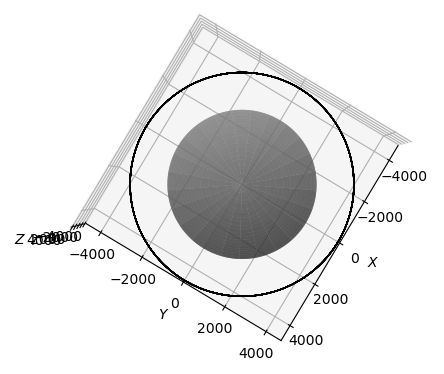
\includegraphics[width=.8\textwidth]{Im/luz_circular.png}
    \caption{Órbita circular}
\end{figure}

\begin{figure}[h!]
    \centering
    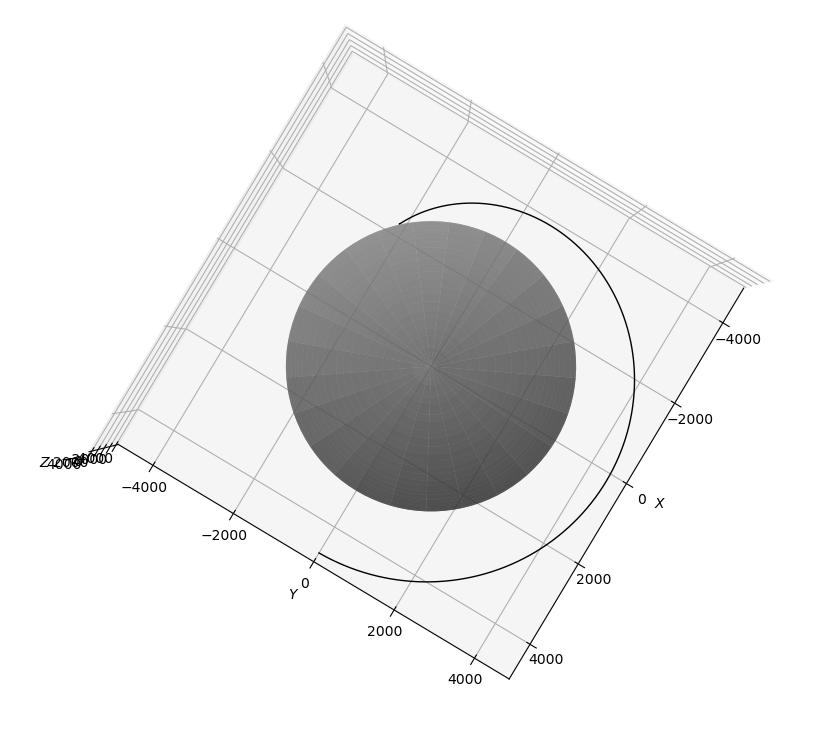
\includegraphics[width=.8\textwidth]{Im/luz_interior_angulo91.png}
    \caption{Desviación de 1° la órbita circular hacia el interior}
\end{figure}

\begin{figure}[h!]
    \centering
    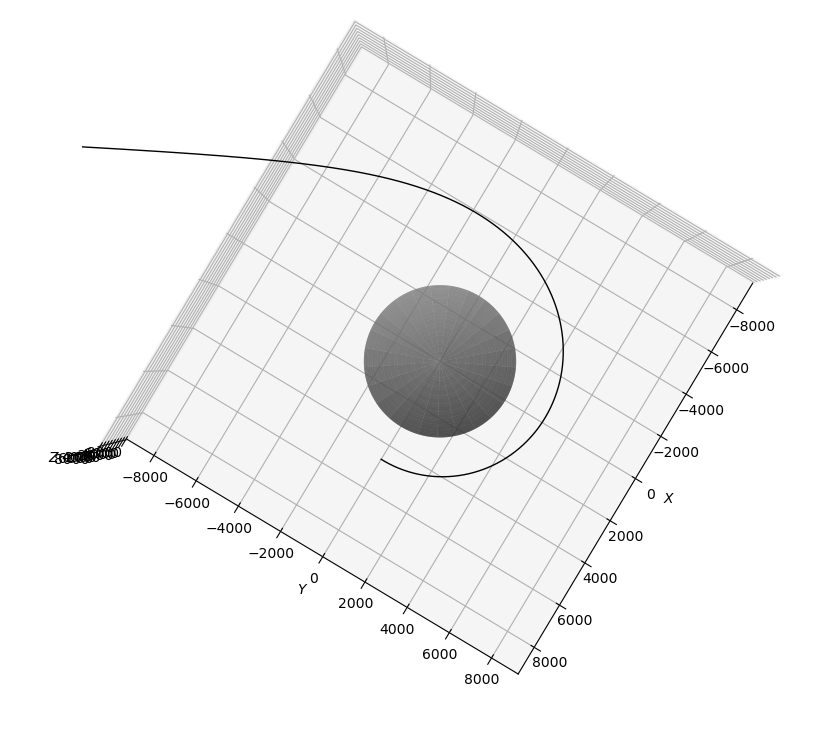
\includegraphics[width=.8\textwidth]{Im/luz_exterior_angulo89_1vuelta.png}
    \caption{Desviación de 1° de la órbita circular hacia el exterior}
\end{figure}

\newpage
\subsection*{\textbf{Órbita de Mercurio}}
Uno de los grandes problemas que tuvo la Mecánica Newtoniana es explicar las observaciones respecto a la precesión del perihelio de Mercurio: La teoría predecía una precesión de $531.9\ arc seg/siglo$, mientras que las observaciones medían $575\ arc seg/siglo$ ¡Una diferencia de $43\ arc seg/siglo$! Pasaron décadas hasta que al fin la teoría de la Relatividad General de Einstein mostró que al considerar la curvatura del espacio-tiempo debido al sol, Mercurio precesa aproximadamente $43\ arc seg/siglo$. Y, añadiéndole la contribución de los otros planetas del sistema solar se termina de explicar las observaciones. Simulamos una partícula partiendo del perihelio de mercurio, moviéndose con velocidad radial nula y velocidad tangencial máxima. Las condiciones iniciales\footnote{https://nssdc.gsfc.nasa.gov/planetary/
factsheet/mercuryfact.html} son:
\begin{equation}
    r_{inicial}=46.002x10^6 Km\ \text{, }\ \Vec{V}= 0\Vec{e}_r + (58.98 m/s)\Vec{e}_{\phi}
\end{equation}

\begin{figure}[h!]
    \centering
    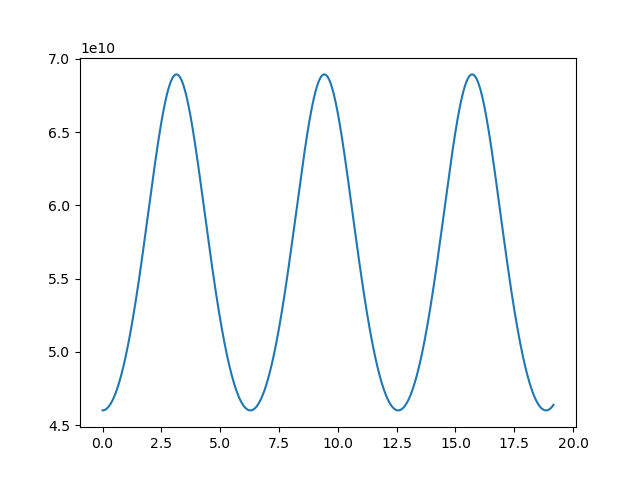
\includegraphics[width=.8\textwidth]{Im/rvsphi_mercurio.png}
    \caption{Gráfica de la órbita de Mercurio: $r$ vs $\phi$}
\end{figure}

Midiendo a que ángulos se dan los mínimos, los perihelios, y viendo la diferencia de esos ángulos se puede estimar la precesión del perihelio. Con la precisión que tenemos, este número nos varía entre la mitad del valor real, y el doble del valor real. 

\begin{figure}[h!]
    \centering
    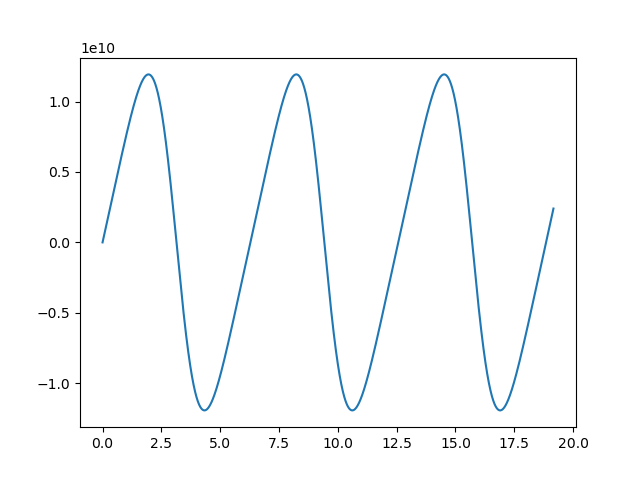
\includegraphics[width=.8\textwidth]{Im/drvsphi_mercurio.png}
    \caption{Gráfica de $\frac{dr}{d\phi}$ vs $\phi$}
\end{figure}

\subsection*{Muchas posibilidades}
Bajo ciertas limitaciones computacionales, es posible jugar con cualquier condición inicial. Dejamos una genial:

\begin{figure}[h!]
    \centering
    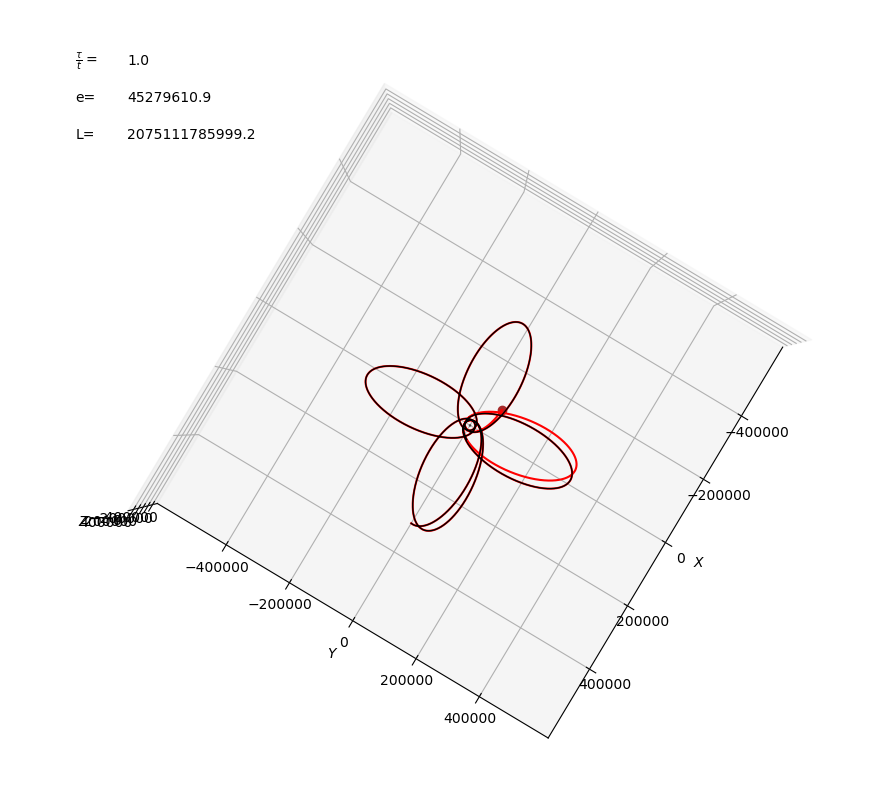
\includegraphics[width=.8\textwidth]{Im/Roseta.png}
    \caption{Órbita divertida en forma de flor.}
\end{figure}
\newpage


